\documentclass{article}
% Formatting-this makes it a full page
\usepackage[margin=1in]{geometry}
%This allows you to use most math symbols
\usepackage{amsmath,amsfonts,amssymb,mathtools}
%This package, and the following lines, allow you to define lemmas, corollaries, theorems, and examples.  
\usepackage{amsthm}
\title{Math 263: Homework 1}
\author{Fangzheng Yu}
\date{\today}
\begin{document}
%Makes the title show up!
    \maketitle
    \begin{enumerate}
        %question1
        \item
        \begin{enumerate}
            %question1_a
            \item The number is: 
            \begin{align*}
                \frac{9!}{2!3!} = 30240
            \end{align*}
            %question1_b
            \item 
            If ``O'' is on the start and end, the number of ways:
            \[\frac{7!}{3!}\]
            
            If ``E'' is on the start and end, the number of ways:
            \[\frac{7!}{2!}\]
            
            Thus, The number is:
            \begin{align*}
                \frac{7!}{3!} + \frac{7!}{2!} = 3360
            \end{align*}
        \end{enumerate}
        %question2
        \item 
        Imagine the three sisters to be a person,
        so there is ``7'' persons now.\\
        Order the ``7'' group at first \((7!)\),
        and then order in the ``3'' group \((3!)\).\\
        The number of the ways is:
        \[7!3! = 30240\]
        %question3
        \item 
        \begin{enumerate}
            %question3_a
            \item The number of ways is:
            \[\binom{2}{1} \binom{5}{1} \binom{6}{1} \binom{9}{3} = 5040\]
            %question3_b
            \item If we exclude the situation in question \((a)\) from the whole situation,
            we would get the answer.\\
            The number of ways is:
            \[\binom{11}{5} \frac{5!}{3!} - 
            \binom{2}{1} \binom{5}{1} \binom{6}{1} \binom{9}{3} = 9240 - 5040 = 4200\]
        \end{enumerate}
        %question4
        \item The number of ways is: 
            \[\binom{4}{8} - \binom{6}{2} = 70 - 15 = 55\]
        %question5
        \item 
        \begin{enumerate}
            %question5_a
            \item The number of shortest paths:
            \[\binom{6}{3} = 20\]
            %question5_b
            \item The number of shortest paths:
            \[\binom{6}{3} - \binom{3}{1} \binom{3}{1}\ = 20 - 9 = 11\]
            %question5_c
            \item 
            \begin{proof}[proof1]
                Imagaine that we have a $n$ x $n$ grid.\\
                And the left in the equation is the number of the distinct shortest ways that a point moves from A to B.\\
                And the right is the number of the distinct shortest ways that a point moves from A to B and pass through C.
                C is point whose horizontal distance is $(n - i)$ and veritcal distance is $i$. And $i$ is an integer ranging from 0 to $n$,
                so C can be all the point on the grid's diagonal. (As shown in the figure~\ref{fig:Drawing})
                And it is clear that if the point moves from A to B, it must pass some of the point on the grid's diagonal. Thus, the right equals left.
                \textbf{\textit{i.e.}} $\sum_{i = 0}^n \binom{n}{i} \binom{n}{n - i} = \binom{2n}{n}$.
                    \begin{figure}
                        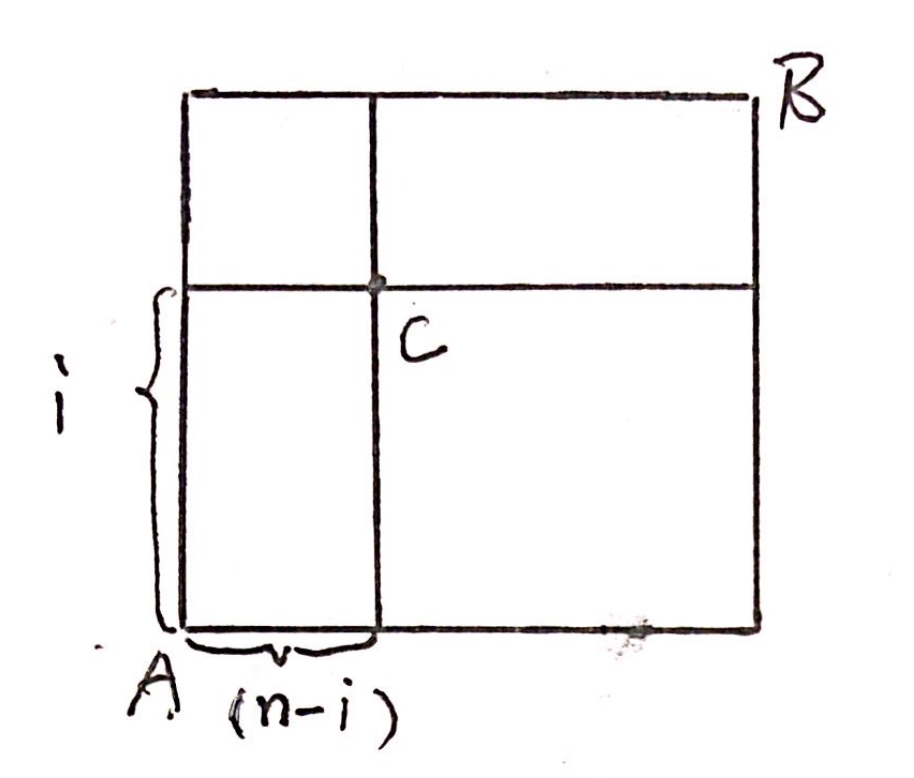
\includegraphics[width=2in]{Drawing}
                        \centering
                        \caption{point c and n-by-n grid}
                        \label{fig:Drawing}
                    \end{figure}
            \end{proof}

            \begin{proof}[proof2]
                Consider we have a polynomial $(x + 1) ^ {2n}$,
                and we want to get the coefficienct of the item whose power is $n$. It is clear that the coefficient of x with power of n is $\binom{2n}{n}$.\\
                We can view the equation as $(x + 1) ^ n (x + 1) ^n $.
                In this two separate polynomial, let the power of x in the first polynomial is $i$, so the second is $n - i$.
                And the coefficienct for the first is $\binom{n}{i}$, and the second is $\binom{n}{n - i}$.
                So we can get the item $\binom{n}{i}x^i \binom{n}{n - i}x^{n - i}$, which contains x with power of $n$.
                And then if sum all this coefficiencts, we get $\sum_{i = 0}^n \binom{n}{i} \binom{n}{n - i}$.\\
                Thus, $\sum_{i = 0}^n \binom{n}{i} \binom{n}{n - i} = \binom{2n}{n}$. 
            \end{proof}
        \end{enumerate}
        
    \end{enumerate}
\end{document}